\chapter{Migration}

	In dem vorherigen Kapitel wurden Module und ihre Eigenschaften, Konstruktionsregeln sowie Modularten behandelt. Dieses Kapitel beschäftigt sich mit der Fragestellung, wie Altsysteme, die vor dem Modulsystem von Java entwickelt wurden, in dem Modulkontext betrieben werden können und was getan werden muss, um diese den modernen Anforderungen anzupassen und zu modularisieren.\bigbreak

	Die Migration behandelt Systeme, die nicht beständig auf dem aktuellen Stand der Technik gehalten werden können und an ihren Ausführungskontext gebunden sind. Diese rutschten langsam in den Bereich der Altsysteme, bis ihr Lebenszyklus zu Ende geht und der Legacy-Zustand erreicht ist. Um die Systeme weiterhin zu nutzen, müssen sie in eine Umgebung mit den geforderten Eigenschaften, ohne Änderungen der internen Struktur vorzunehmen, übertragen werden. Dieses Verfahren wird oft im Bereich der Softwaretechnik mit Software Reengineering und Software Neuimplementation verwechselt, dessen Ziel in der Optimierung der Codebasis liegt und nichts mit dem Ausführungskontext zu tun hat. \cite{martens2016ablosung} \bigbreak

	% Migrationsmethoden und der von ihnen gelösten Problemen. 
	Während des Betriebs einer lang gepflegten Kernapplikation, wird der Lebenszyklus öfter überschritten und muss den Migrationszyklus mehrmals durchlaufen. Zum Beispiele kann eine Applikation an Größe gewinnen und muss in die Cloud ausgelagert werden, die Anforderungen können sich verschieben und der Technologie-Stack muss an die Marktbedürfnisse angepasst werden, darüber hinaus kann der Ausführungskontext einen großen Versionssprung hinter sich lassen, der das Warten der Software unter den momentanen Bedingungen unmöglich macht. \newline
	Dem zufolge ist das Umfeld der Software Entwicklung eine dynamische Umgebung, denn auch mit einer gut durchdachten Architektur kann nicht garantiert werden, dass in der Zukunft heutige Paradigmen, Werkzeuge und Aufgabenbereiche denselben Kurs behalten. Deswegen existieren bereits sämtliche Migrationsstrategien, die als ein Leitfaden den Entwickler durch die Migration führen. \bigbreak

	Im folgenden Kapitel werden Ansätze vorgestellt, die Monolithische- sowie Bibliotheksanwendungen in das modulare System überführen ohne Änderung an der internen Funktionalität durchzuführen. 


\section{Legacy-System}

	Der Begriff \textit{Legacy-System} beschreibt ein altes System, das innerhalb einer Organisation länger als der geplante Lebenszyklus in Betrieb bleibt. Der englische Begriff \textit{Legacy}, zu Deutsch Erbe, bezieht sich nicht auf das Alter der Software, sondern auf die Interpretation der Software als Erbe. Da die Umsetzung von früheren Entwickler Teams durchgeführt wurde, die sich an damaligen Konzepten und Strategien bedienten, ergab die Lösung ein Erbe mit bestimmten Einschränkungen, die für die zukünftige Erweiterung der Software eine große Rolle spielen. Denn die typischerweise veralteten Verfahren und Technologie lange Lebenszyklen mit umfangreichen Veränderungen und Erweiterungen erfahren haben \cite{sneed2016softwaremigration}. \bigbreak

	Zu meist handelt es sich um sogenannte Kernsysteme zur Unterstützung wesentlicher Geschäftsprozesse eines Unternehmens. Sie sind in der Regel geschäftskritisch und können nicht ohne großen Aufwand und Risiko für das Unternehmen ausgetauscht werden. Aufgrund ihres langen Lebenszyklus, ihrer Komplexität und ständigen Überarbeitungen, ist die Logik solcher Systeme oft unübersichtlich und schlecht dokumentiert. Ihre Implementierung kann zusätzlich früher geltenden Standards unterliegen und anderen Programmierparadigmen folgen, die nur schwer verständlich sind. Daher sind Geschäftsprozesse und Geschäftsregeln im Code versteckt und müssten z.\,B. für eine Neuimplementation erst rekonstruiert werden \cite{martens2016ablosung}.

\section{Migration} \label{ssub:migration}

	% schau in diesem buch nach einer defenition  mit den storchen 
	Die Softwaremigration bezeichnet die Überführung eines Softwaresystems in eine andere Zielumgebung oder in eine sonstige andere Form, wobei die fachliche Funktionalität unverändert bleibt. Als Ausgangspunkt steht dabei immer ein bestehendes System, das an Anforderungen und Techniken des Anwendungsbereiches angepasst werden muss \cite{sneed2016softwaremigration}. Die Adaption an den neuen Anwendungsbereich geschieht zu meist nicht problemlos und muss system- und kontextbezogene Hürden überwinden. 

\section{Migrationshürden} \label{MigH}

	% Einleitung: hier kommen allgemeinen Beispiele der Migrationsproblematik 
	Die Migrationshürden sind fest mit dem Anwendungskontext verbunden und hängen stark von der Beschaffenheit der neuen Umgebung ab. Da in unserem Fall die Migration innerhalb der Java Umgebung stattfindend, müssen die Neuerungen des Modulsystems analysiert und auf den bestehenden Zustand der Applikation abgebildet werden.\bigbreak

\begin{itemize}
	% Hauptteil: Probleme und Hürden, die der neue Kontext macht
	\item Die Probleme des Modulsystems beginnen mit den Zugriffsrechten auf die Core-JDK API's. Diese sind ab sofort in dem Modul gekapselt und bieten nur eingeschränkte Möglichkeiten Aufrufmöglichkeiten. Nichtsdestotrotz stellt Java für viele der gekapselten API's einen Ersatz zur Verfügung, wodurch zahlreiche Probleme mit einem relativ geringen Aufwand behoben werden können. \cite{masteringJava9,modulProgJava9,modulMitJava9,javaMod9} 


	\item Im Weiteren verbietet das neue Modulsystem namensgleiche Pakete in verschiedenen Modulen. Dieses adressiert das vorher besprochene Problem aus dem Kapitel \ref{sec:nam}, nämlich den Zugriff auf privat deklarierte Pakete aus fremden Modulen. Trotzdem gibt es Bibliotheken mit ähnlicher Paketstruktur, die sich nicht böswillig sich Zugriff verschaffen wollen, sondern spiegeln eine Standardstruktur einer Bibliothek widerspiegeln, wie zum Beispiel \textit{de.firma.input.reader} kann in mehreren Bibliotheken eines Unternehmens existieren kann und ab Java 9 nicht mehr zulässig sein wird. Somit müssen Module mit ähnlicher Struktur angepasst werden, um den nächsten Modularisierungsschritt durchführen zu können. \cite{masteringJava9,modulProgJava9,modulMitJava9,javaMod9} 


	\item Der Klassenlader-Typ des Applikation-Klassenladers wurde überarbeitet und infolgedessen auch das Arbeiten mit den ehemaligen URL-Klassenlader Methoden. Der bestehende Code, der den URL- Klassenlader exzessiv nutzt und zum Beispiel Ressourcen aus verschiedenen Quellen lädt, muss auf den \textit{Secure-Klassenlader} oder  \textit{Klassenlader} aufgewertet werden, um funktionstüchtig zu bleiben. \cite{oracModClassLoader,jecan2017java} 


	\item Einer der kritischen Veränderungen, die die Modultatform mit sich bringt, ist das Verbot von zyklischen Abhängigkeiten von Modulen untereinander. Diese dürfen sich nicht gegenseitig mit dem Schlüssel \textit{require} koppeln, da sonst eine Veränderung in einem Modul zwangsläufig eine Änderung in den anderen Modulen hervorrufen kann. Dieser Stil kann sich schnell über die ganze Applikation verbreiten und kleine Änderungen an einer Stelle zu unübersichtlichen Seiteneffekten führen. Genau diese Probleme adressiert das Modulsystem in erster Linie und verbietet aus diesem Grund Zyklen in dem Applikationsentwurf. Um bestehende Zyklen in einer Applikation zu lösen, muss die Funktionalität genau betrachtet und in kleine unabhängige Aufgaben aufgeteilt werden. Somit werden Zyklen aufgebrochen und die Aufgabenstellung jedes Moduls klar definiert. \cite{java9modRevealed,modulProgJava9,modulMitJava9} 
\end{itemize}

\section{Migrationsarten} \label{Migratiosarten}

	% Schluss: Bewegen uns auf die möglichen Migrationsstrategien für die Modularisierung.
	Da jede Applikation spezifisch Migrationsanforderungen besitzt, gibt es unterschiedliche Verfahren, die sich bestimmten Kriterien widmen. Dementsprechend sollte man die gegebene Applikationsbeschaffenheit ermitteln und dessen Probleme auf die passende Migrationsstrategie abbilden. Die prominenten Migrationsstrategien der Software Techniken sind \textit{Chicken Little} und \textit{Butterfly}, zwei der gängigsten Arten der Softwaresystem Migration. \cite{sneed2016softwaremigration} \bigbreak


	% Chicken Little
	Softwaresysteme, die nach dem \textit{Chicken-Little-Ansatz} migriert werden, zerlegen das System in mehrere Migrationspakete, die einzeln in kleinen inkrementellen Schritten in die neue Zielumgebung überführt werden. Damit der Betrieb des Systems nicht für die Zeitdauer der Migration ausfällt, existieren alte, neue und migrierte Teilsysteme nebeneinander. Die korrekte Kommunikation der Softwarebausteine muss über entsprechende Kommunikationskanäle errichtet werden und gestaltetet damit eine Brücke zwischen Alt- und Neuentwicklung, die zusammen eine gemeinsame Ressourcenbasis nutzen können. \cite{sneed2016softwaremigration} \bigbreak

	% Butterfly 
	Der \textit{Butterfly-Ansatz} geht von einer separaten Entwicklung der Applikation in der neuen Umgebung aus. Dies hat zur Folge, dass die Altapplikation in Betrieb bleibt und unverändert ihre Aufgabe erfüllt, bis der Nachfolger, der parallel zu dem Betrieb entwickelt und getestet wird, die Funktion korrekt widerspiegeln kann. Im Anschluss werden Ressourcenbestände in kleinen Paketen an die Applikation im neuen Kontext transferiert und das Altsystem abgeschaltet. Das Butterfly-Verfahren vermeidet also während der Migration den simultanen Zugriff auf Legacy- und Zielsystem. \cite{sneed2016softwaremigration} \bigbreak

	% Ein text der auf die nächsten Kalitel einführt 
	Zwischen den beiden vorgestellten \textit{Migrationsideen} hat sich das Java Team für die Unterstützung der Schrittweise-Migration entscheiden, die eine Applikation in kleine Softwareeinheiten aufteilt und langsam auf den neuen Modulpfad migriert. Der parallele Betrieb der neuen sowie alten Struktur wird durch eine interne Brücke, die korrekte Kommunikation zwischen den Klassenpfad und den Modulpfad errichtet umgesetzt. Die Implementation der Kommunikationsbrücke und ihrer Charakteristika, die eine kritische und verantwortungsvolle Aufgabe in dem Migrationsprozess trägt, wird für uns von dem Java Team zur Verfügung gestellt. Somit unterstützt und führt das Modulsystem von Java den Entwickler bei der Hand zu der korrekten, sicheren, modernen und funktionstüchtigen Modularchitektur. \newline
	Ungeachtet dessen, ist die Migration einer Applikation zu diesem Zeitpunkt nicht zwingend und kann innerhalb des Modulsystems weiterhin betrieben werden, da diese keine speziellen Hilfsmittel von der Umgebung fordern.\bigbreak

	In den nachfolgenden Kapiteln werden unterschiedliche Varianten der Migration und des Betriebs einer Applikation innerhalb des Modulsystems vorgestellt. 


\subsection{Plattform Migration}
	Die simpelste Migration ist eine reine Plattform Migration, ohne Änderungen an der Software vorzunehmen, wie in der Abbildung \ref{fig:PM} dargestellt. Dies ist möglich, dank der Unterstützung des Klassenpfades, der in diesem Fall die Applikation als ein \textit{unbenanntes Modul} im Modulsystem betreibt. Wie bereits im Kapitel \ref{Modularten} angesprochen, bietet dieses Modul den Betrieb der Legacy Anwendung in der neuen Umgebung mit dem geringen Anteil der möglichen Vorteile, wie zum Beispiel den Sicherheitsupdates. Zusätzlich behält die Applikation ihre monolithische Architektur und vermisst alle Modulsystem Features, die im Kapitel \ref{sec:ZdM} und \ref{sec:ME} angesprochen wurden.

	\begin{figure}[h]
		\centering
	    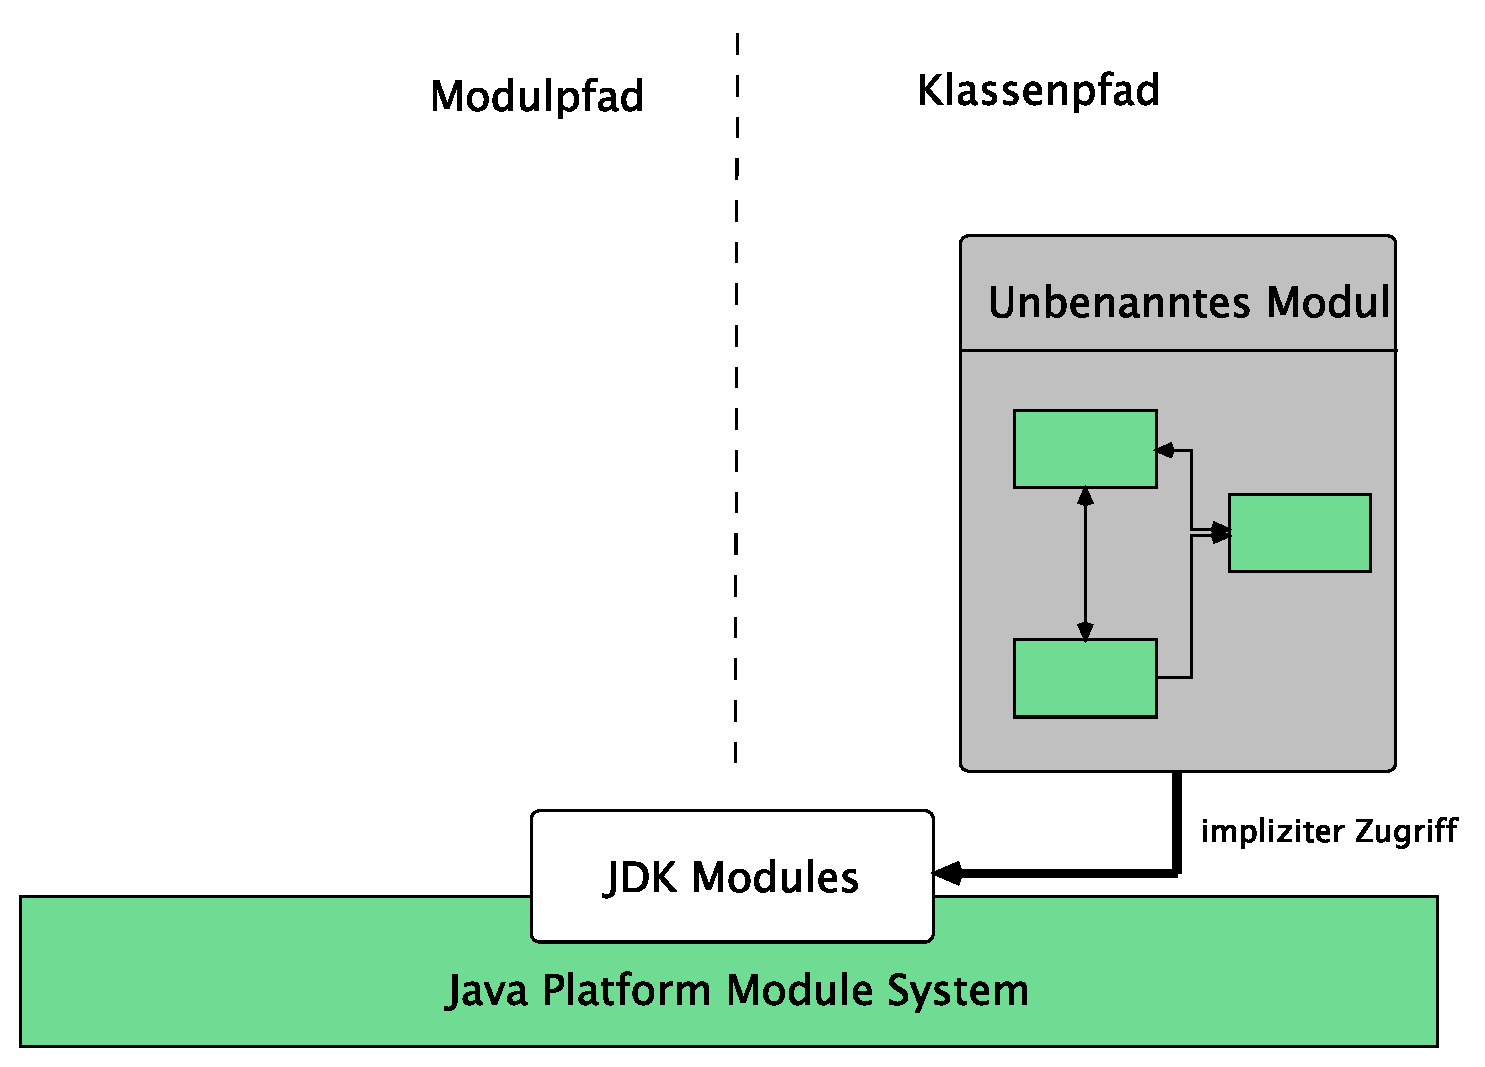
\includegraphics[width=0.8\textwidth]{material/images/platform-migrate.pdf}
	    \caption{Plattform Migration \cite{modulMitJava9}}
	    \label{fig:PM}
  	\end{figure}

	Eine weitere Möglichkeit wäre es, die Applikation und ihre Bibliotheken auf den Modulpfad zu migrieren und als \textit{automatische Module} zu betreiben. Somit wäre der alte Klassenpfad  nicht mehr im Applikationsdesign vorgesehen und fokussiert die Entwickler auf die Arbeit mit dem Modulpfad. Dennoch lässt sich nicht jede Anwendung in diesem Still migrieren, denn die Hürden aus dem Kapitel \ref{MigH}, wie die \textit{Zyklenfreiheit} sowie das Verbot der \textit{Split-Packages} in Legacy-Bibliotheken nicht immer gegeben ist. 



\subsection{Top Down Migration}
	Die \textit{Top-Down} Migration behandelt die Migration von oben nach unten, dabei werden zuerst die Applikation und im Nachhinein die Drittanbieter-Bibliotheken migriert. Dafür müssen die Applikationspakete auf Abhängigkeiten geprüft und entsprechende Module sowie Modulbeschreibungen nach den im Kapitel \ref{sec:MEK} besprochenen Kriterien erstellt werden. Mit dieser Methode werden die Drittanbieter Bibliotheken zuletzt betrachtet, da es sich bei diesen um Fremdcode handelt. \newline
	Da nach der Prüfung der Abhängigkeiten ein Graph entsteht, verweist dieser ab einem gewissen Punkt auf die Bibliotheksabhängigkeit der Applikation, die wiederum von weiteren Bibliotheken abhängen. Somit kann die Wurzel der benötigten Drittanbieter-Bibliotheken einer Applikation ausfindig gemacht und als \textit{automatische Module} in den Modulpfad eingebunden werden. Somit können diese, wie bereits in im Kapitel \ref{Modularten} behandelt, sowohl mit der Applikation als auch mit den Legacy Elementen ihrer eigenen Abhängigkeiten zugleich interagieren. Zum Schluss kümmert man sich um die Bibliotheken auf dem Klassenpfad, indem diese ersetzt oder selbständig weiterentwickelt werden, mit dem Ziel die Gesamtapplikation auf dem Modulpfad zu übertragen. \cite{javaMod9,modulProgJava9,java9modRevealed,modulMitJava9,masteringJava9}\bigbreak
	\begin{figure}[h]
		\centering
	    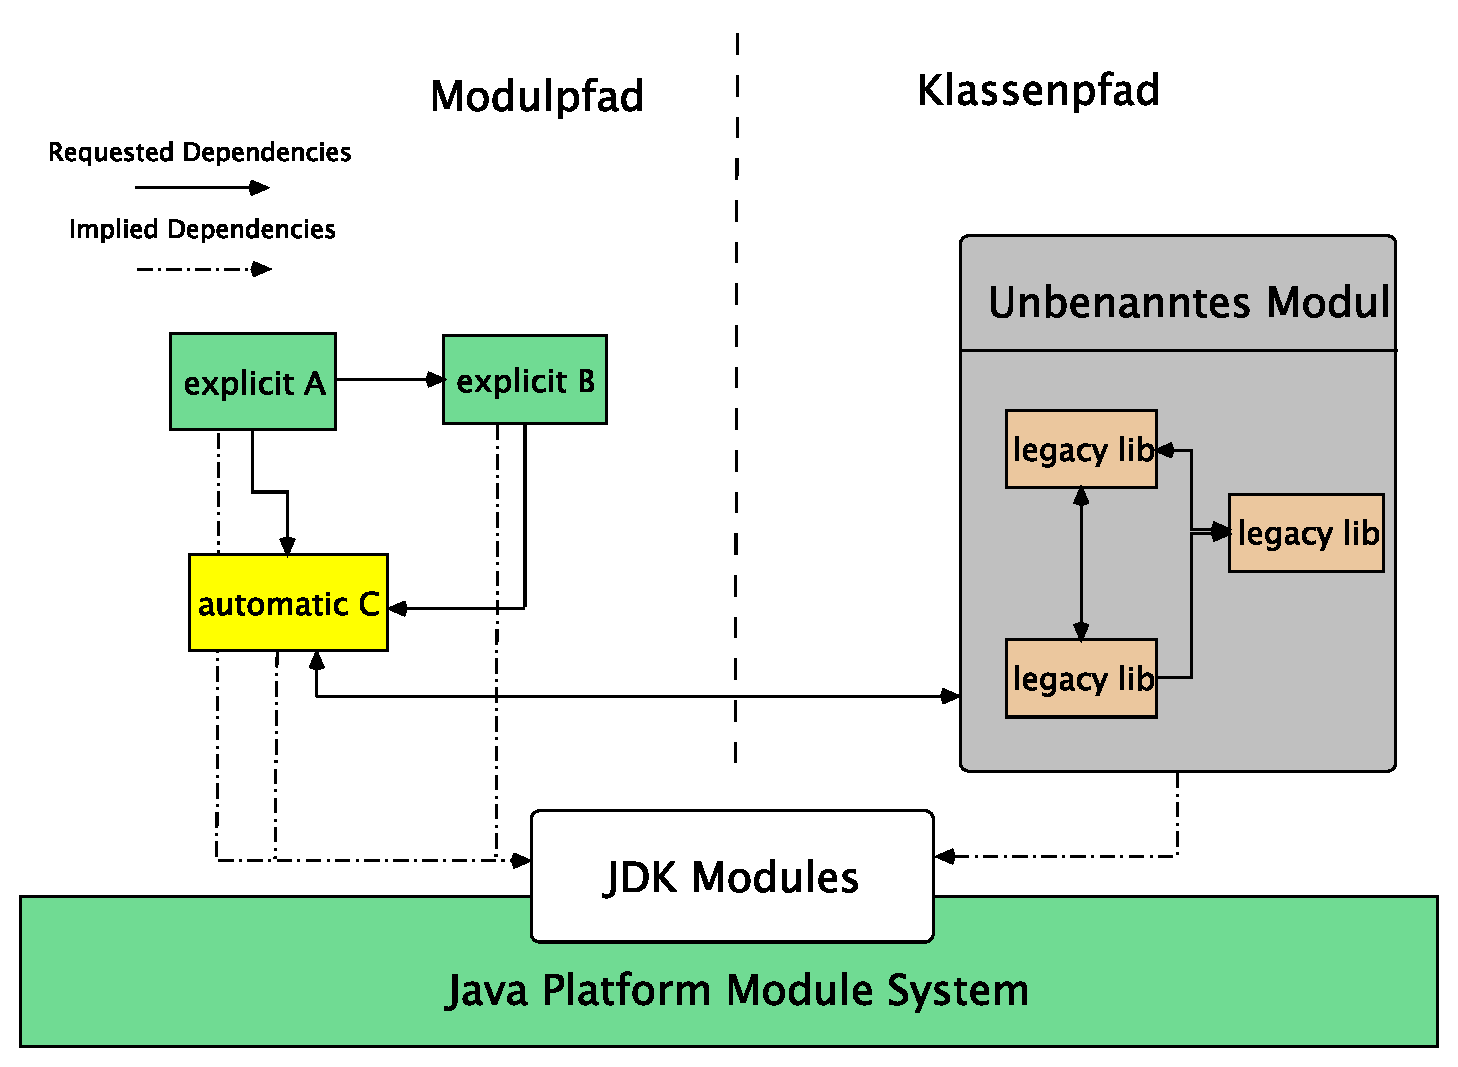
\includegraphics[width=0.8\textwidth]{material/images/top-down-migrate.pdf}
	    \caption{\textit{Top Down} Migration}
	    \label{fig:TDM}
  	\end{figure}

	Diese Migration ist besonders vorteilhaft bei Applikationen, die eine geringe Codebasis besitzen und in einem kurzen Zeitraum eine modularisierte Form annehmen können. 

\subsection{Bottom Up Migration} \label{sec:bottomUP}
	Die \textit{Bottom Up} Migration behandelt lose Module zuerst, denn diese haben keine Abhängigkeiten und bieten eine gekapselte Funktionalität an. Um herauszufinden, welche Module sich für den initialen Migrationsschritt eignen, kann der Abhängigkeitsgraph mithilfe des \textit{JDepth} erstellt werden. Module, die als Blätter aufzufinden sind, können zuerst migriert werden, da sie keine Kinderknoten und somit keine Abhängigkeiten besitzen. Im weiteren Verlauf der Migration werden die übrig gebliebenen und neu entstandenen Blätter des Abhängigkeitsbaums abgearbeitet, bis die ganze Applikation, samt der Drittanbieter Bibliotheken, sich auf dem Modulpfad befindet. Während der Migration müssen natürlich die im Kapitel \ref{sec:MEK} besprochenen Kriterien erfüllt werden, um eine robuste Umsetzung zu erreichen. \cite{javaMod9,modulProgJava9,java9modRevealed,modulMitJava9,masteringJava9} \bigbreak
	\begin{figure}[h]
		\centering
	    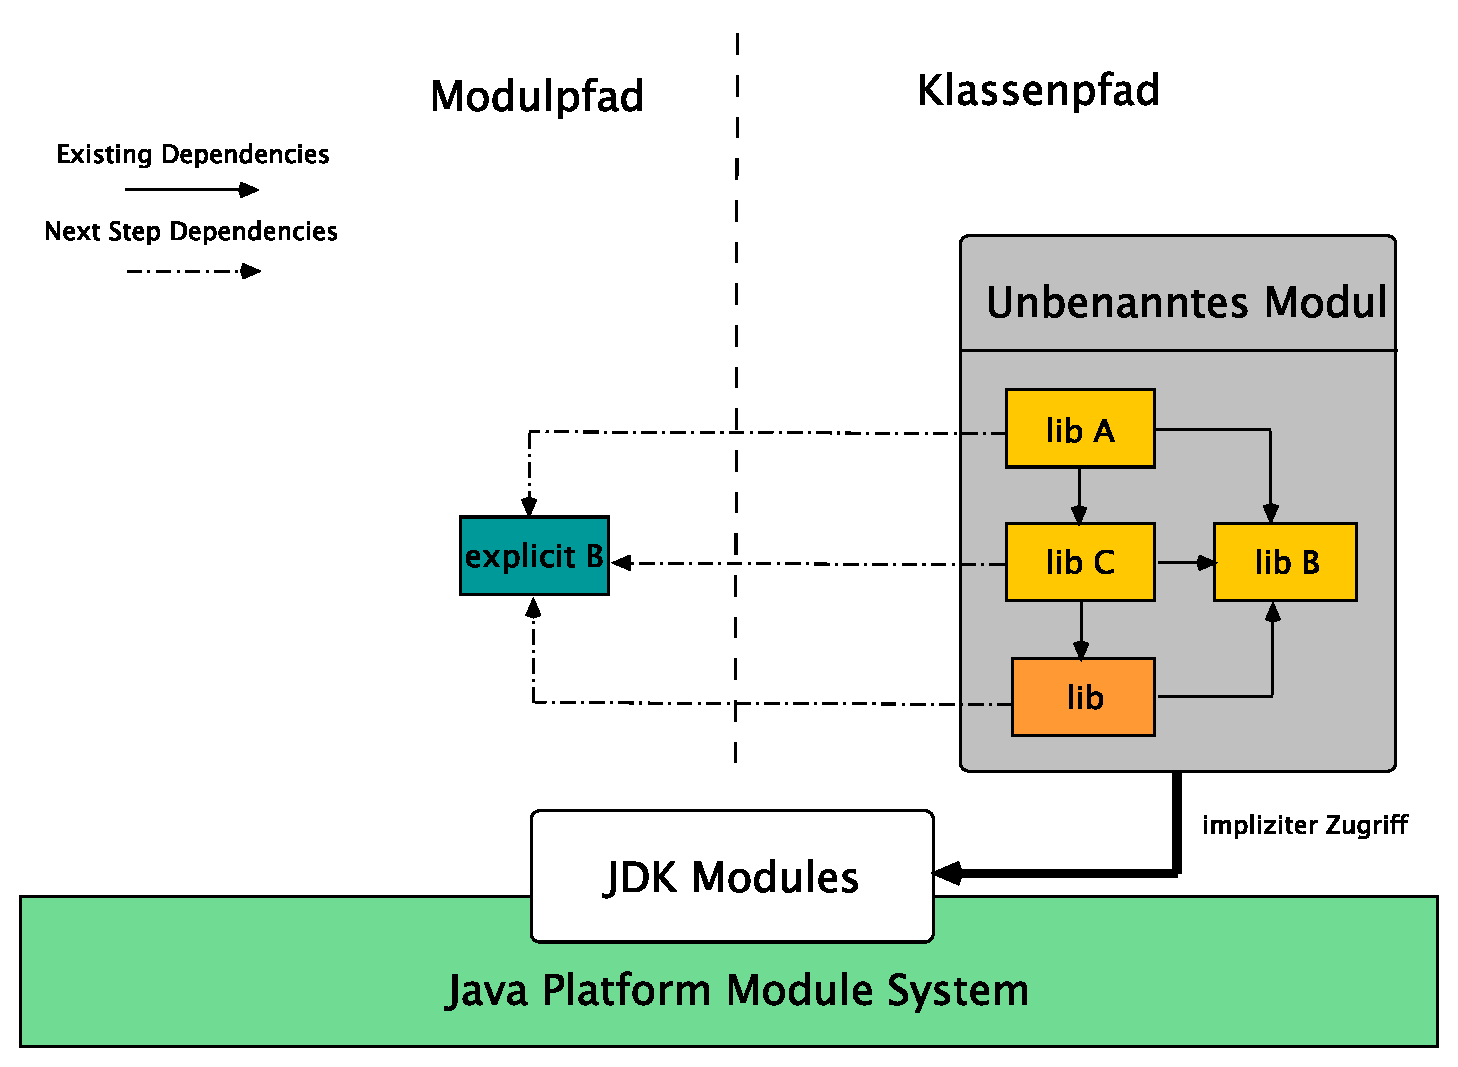
\includegraphics[width=0.8\textwidth]{material/images/bottom-up-migrate.pdf}
	    \caption{\textit{Bottom Up} Migration \cite{modulMitJava9}}
	    \label{fig:BUM}
  	\end{figure}
	In der Abbildung \ref{fig:BUM} wird der erste Schritt der \textit{Bottom Up} Migration angedeutet, indem die \textit{lib B} als erste auf den Modulpfad migriert wird. Diese hat keine Abhängigkeiten und ist der perfekte Kandidat für den initialen Schritt. Als Nächstes bietet sich die \textit{lib} Bibliothek für die Migration an, da sie keine weiteren Abhängigkeiten in den Klassenpfad besitzt. Jedoch ist sie eine Drittanbieter Bibliothek und kann von uns nicht bearbeitet werden. Aufgrund dessen wird die \textit{lib C} für  den nächsten Migrationsschritt ausgewählt und als ein \textit{automatisches Modul} auf den Modulpfad migriert. Somit kann dieses die \textit{lib} und \textit{lib B} zugleich nutzen. Als Nächstes ist die \textit{lib A} an der Reihe, dessen komplette Abhängigkeiten sich bereits auf dem Modulpfad befinden. In der Konsequenz befinden sich alle Applikationsbibliotheken auf dem Modulpfad. \cite{javaMod9,modulProgJava9,java9modRevealed,modulMitJava9,masteringJava9} \bigbreak

	Die \textit{Bottom Up} Migration bietet sich bei bereits aufgeteilten Applikationsarchitektur an, die über eine Menge von \textit{Jar} Bibliotheken betrieben wird. Diese braucht weniger Aufwand, um den Monolithen zu zerlegen und sind bereits über Schnittstellen miteinander Verbunden. \cite{modulProgJava9,modulMitJava9}








